\appendix
\section{Gregor -- The Twisting Bezier Spline Editor}\label{Chapter:Gregor}
\subsection{Introduction}
{
    ``Gregor'' is an open source software developed specifically as a minimalist editor for the twisting bezier splines. A complete user manual be viewed online [cite] but the main features are discussed here. The most fundamental user requirements are very simple.
    \begin{itemize}
      \item
      {
        The most fundamental requirement was that the tool be able to let the user graphically draw a rotating bezier spline. It was not only convenient but also logical to make the editing sequence similar to other vector editing software. This will make the transfer easier for people who already have some experience in other applications.
      }
      \item
      {
        The application must be able to save and load the edited work using a data file.
      }
      \item
      {
        The user should be able to drag and zoom the view port using the mouse cursor and keyboard shortcuts.
      }
      \item
      {
        There should be a provision to load images into the workspace so that they can be traced.
      }
    \end{itemize}
}
\subsection{Overview of the implementation}
{
    Gregor provides the minimal functionality to work with twisting bezier splines. Additionally, many of the secondary features were implemented to fulfil the needs of actual artists who found the basic interface too wanting. Microsoft .Net framework was chosen to construct the GUI application mainly because it supports writing code in Microsoft Visual C Sharp (C\#) and because all the intended features like mouse and keyboard interactions and graphics are easy to implement in it. Gregor can create, modify, import and save twisting splines. it mainly consists of a single \emph{Windows Form} that hosts the basic editing and viewing controls and an interactive workspace. The workspace is a virtual page that can be zoomed into and panned around using the cursor and keyboard shortcuts. One can change the viewing modes of the workspace to better suite the editing needs. One can choose to display or hide certain anchors, ink-marks, curvature spline, and change the appearance of a twisting spline. To assist the user, Gregor also allows to import and scale images that can be used to trace twisting bezier splines.

    See Appendix \ref{Appendix:Gregor} that describes the interface, enlists the features and describes the usage of most important parts of the application.
}
\subsection{Interface}
{
    The view of the software is the spline editor with a detailed main menu as shown in Fig. \ref{Fig:GregorInterface}, document summary and a list of most commonly used toggle buttons. The application also provides some keyboard shortcuts for the most frequently used toggle options like changing the visibility of different elements and toggling the editing modes.

    The information a rotating spline contains is too much to be viewed simultaneously. The center point of the anchors, the curvature handles, twist handles, the curve, the inkmark and the background image, when displayed simultaneously is just chaotic. On top of that, when all of these elements are interactive, using a single mouse cursor to interface becomes a headache. This is why the application presents viewing and editing modes.
    \subsubsection{The Viewing Modes}
    {
        The viewing modes can be controlled using options (g1) through (g3) as shown in Fig.  \ref{Fig:GregorInterface}, the ``View'' menu (a2), or the keyboard shortcuts. There are essentially three modes of view.
        \begin{itemize}
          \item (g1) is ink and curve mode. In this mode, the splines curves and the selected handles will be shown alongwith the ink marks.
          \item (g2) is ink-only mode. In this mode, the curvature handle of the splines alongwith the anchors and the handles are hidden.
          \item (g3) is curve-only mode. The inkmark will be hidden in this mode and only the curve alongwith the selected handles will be visible.
        \end{itemize}
        it is obvious that only one mode can be activated at a moment and it can be selected either from the options (g1) through (g3) in Fig.  \ref{Fig:GregorInterface} or through the View menu. Instead of clicking on the toggle buttons, using the keyboard shortcuts can sometimes be even more convenient.
    }
    \subsubsection{The Editing Modes}
    {
        The editing models enable or disable the anchors, curvature handles and the twist handles. As shown in Fig. \ref{Fig:GregorInterface} (h1) through (h3), the editing mode toggle buttons can be used to enable or disable any of these handles. Just like the editing modes, these modes can also be controlled using the keyboard shortcuts. Unlike the viewing modes, however, these modes can be enabled all at a time. It must be noted that while in ink-only mode, none of the editing modes will have any effect of the usability of the editing handles.
    }

    \begin{figure}
      \centering
      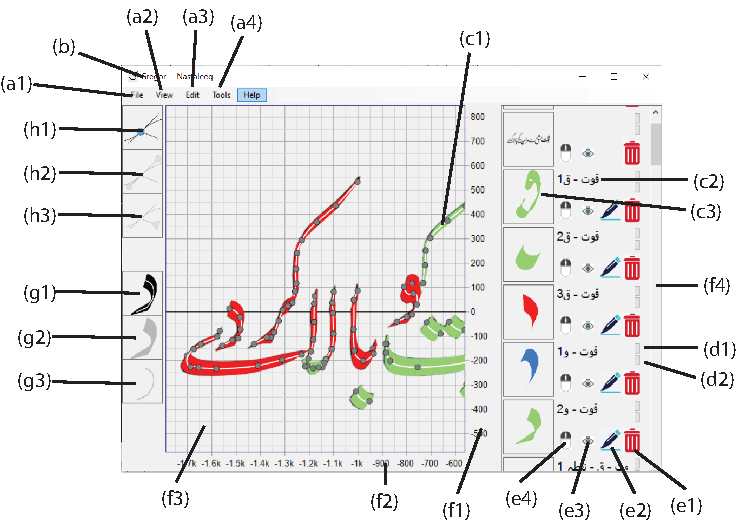
\includegraphics[width=0.9\textwidth]{../Images/GregorInterface.pdf}
      \caption{(a1-a4) The main menu options: (a1) Contains the options to open, save, import, export and clear splines and background images, (a2) enlists some viewing options; the ink viewing modes, visibility different elements of the workspace, visibility of background images, opacity of the ink-marks and rendering algorithm (a3) contains options related to editing on the workspace. It has the option to change the spline editing modes, the behaviour of left click on the workspace, and whether the splines can be dragged or not. (a4) has some analysis tools. (b) is the name of the currently open document. (c) is the main view of each spline in the document, (c2) and (c3) are the name of each spline element and its thumbnail respectively. (d1) and (d2) change the vertical order (z order) of the elements. While hovering the cursor over overlapping splines, the spline with higher position in the list will receive mouse event earlier. (e1), (e2), (e3) and (e4) are used to toggle editability, change visibility, modify color and thickness and delete the respective spline curve respectively. (f1) and (f2) are x and y axis of the workspace. (f3) is the main viewport. (f4) is the list of all the splines and images in the document. (g1) switches the view mode to both spline and inkmark, (g2) changes the viewing mode to ink only. (g3) changes the viewing mode to spline only. (h1), (h2) and (h3) toggle the visibility of center of anchor, curvature handle and the twist handle of the splines.
      } \label{Fig:GregorInterface}
    \end{figure}

}
\clearpage 